\documentclass{article}
\usepackage{graphicx}
\usepackage{color}
\usepackage{url}
\usepackage[font=small,labelfont=bf]{caption}
\usepackage[a4paper, total={16cm, 24cm}]{geometry}
\usepackage{indentfirst}



\begin{document}

\begin{titlepage}
    \begin{center}
        
	\begin{figure}
		\centering
        FACULTY OF MECHANICAL ENGINEERING AND ROBOTICS\\
        AGH UNIVERSITY OF SCIENCE AND TECHNOLOGY\\
        \vspace{0.2cm}
    	\begin{minipage}[b]{0.4\textwidth}
    	    \centering
    		\includegraphics[width=\textwidth]{IMG/AGH.png}
    	\end{minipage}
    	\hfill
    	\begin{minipage}[b]{0.4\textwidth}
	    	\centering
    		\includegraphics[width=\textwidth]{IMG/WIMIR.png}
		\end{minipage}
		\vspace{1cm}
    \end{figure}

    \Huge \textbf{Vision Controlled Mechanical Hand}
        
    \vspace{0.8cm}
    \LARGE 
    \color{black} 
            
    \vspace{0.8cm}       
    \textbf{Damian Durczok\\Mikolaj Gacek\\Adam Kolusz}        
    \vfill       
    \vspace{0.8cm}    
    18.06.2018
        
    \end{center}
\end{titlepage}

\tableofcontents
\break

\section{State of Art}
A typical mechatronic device encompasses many fields of technological engineering. This includes mechanical engineering, electronics, computer engineering, systems and control engineering. To thoroughly design such a system with awareness of all its elements during each step of the process requires the foresight and knowledge of all the components and relations between individual elements. This is the purpose of the state of art - a prerequisite to the initialization of a project. By the end of this section we will have explored existing technologies and solutions to our problem and drawn up a basic model of the mechatronic device.

\subsection{The Problem}
Certain situations that endanger human life benefit from the intervention of a robotic device. However, these robots may be limited in functionality compared to the human counterpart. In cases such as bomb disposal, nuclear power station decommissioning or handling of dangerous substances the dexterity of a human hand is significantly important.

\subsection{The Solution}
The mechanical hand is a device that has been iterated on many times in recent history. Control of such a hand is either by machine or human. For automated tasks, a machine controlled hand is more than sufficient. However, in unpredictable environments human intervention is still necessary.

This is where the idea stems together. A mechanical hand with the full dexterity of its real counterpart controlled in an intuitive way by a human. The control will be based on the idea of mimicking the operators limbs. Pairing this with a strategically placed camera and a virtual reality headset, we have an operator who is fully immersed and in full control of the situation at hand.

\subsection{Mechanical Hand}
Most modern innovations of the mechanical hand are related to the development of prosthetics. BeBionic \cite{bebionic} and Vincent Systems \cite{vincent} among many others have developed such devices that accurately mimic the likeness.

\begin{center}
\includegraphics[width=0.45\textwidth]{IMG/Bebionic_V2_Hand.png}
\captionof{figure}{BeBionic Mechanical Hand}
\end{center}

The most popular actuation method is a combination of a DC motor and either a worm gear or lead screw. The size of the hand leaves us with a very small working area, as a result the driving motors must be very small with high gear reductions.

\begin{center}
\includegraphics[width=0.6\textwidth]{IMG/fingerMech2.png}
\captionof{figure}{Mechanics of a finger \cite{JRRD}}
\end{center}

Another issue to contend with is the weight and speed of the mechanism. For prosthetic use, the hands are made to be lightweight for mobility. Whereas in our application this isn't a problem, we may still benefit from reducing the moments of inertia by increasing the acceleration capabilities of joints. Ideally having the same dynamic properties as the human hand.

The limited working space also forces certain optimization. For instance, not all joints need to be independently driven. We may simplify the model by involving mechanisms that create a fixed relationship between joints.

\begin{center}
\includegraphics[width=0.3\textwidth]{IMG/fingerMech.jpg}
\captionof{figure}{Reducing degrees of freedom mechanically \cite{JRRD}}
\end{center}

A final feature commonly observed is a certain flexion compliance level. Under a certain level of pressure, the joint flexes by either a spring or flexible material. This is a protective measure to prevent the damage of certain elements.

Many hobbyists opt out for a different solution that includes a motor and line. The joints are controlled in one direction by the contraction of a line and in the other by a spring or flexible material. This greatly simplifies the design process by allowing the motors to be located elsewhere. Potentially allowing for much larger drives and a greater gripping force along with greater movement speeds and accelerations. This system also naturally includes flexion compliance.

\begin{center}
\includegraphics[width=0.3\textwidth]{IMG/stringMech.jpg}
\captionof{figure}{Solidworks solution \cite{stringHand}}
\end{center}

This solution isn't as well researched as the earlier method and will require a longer prototyping phase. \\[12pt]
\indent Pneumatics may offer another solution. All the fingers are actuated by a pneumatic air muscle. These prove to have very high grip strength with favourable dynamic characteristics. All however comes with the price of size, to drive such a system a constant supply of compressed air is necessary to accurately position the stroke-length of each air muscle. Additionally a large valve system is necessary to control such a device.

\begin{center}
\includegraphics[width=0.4\textwidth]{IMG/airMuscle.jpg}
\captionof{figure}{Air Muscle}
\end{center}

In summary, we may consider driving our mechanism with either an electric motor or a pneumatic device. The pneumatic device may allow for much better dynamic performance such as limb velocity, acceleration and grip strength. However requires an entire pneumatic system in place which may prove expensive and resource heavy. The DC motor compromises on dynamic performance in place for a more ergonomic design.\\[12pt]
\indent The driving mechanism may be optimized by involving dependent joints. These joints may be driven directly or at a distance using lines. A line driven mechanism alleviates the problem of having to work in a small working area by removing the largest elements externally. 

\subsection{Sensors}
For the human hand to control the mechanical counterpart a set of sensors are necessary. For simplicity, we will only track the position of individual fingers. Although data sets such as grip strength, velocity or acceleration of fingers may inadvertently be natural features of some of the concepts.

A vision system introduces a non-invasive and non-contact method. Free to the public libraries such as OpenCV paired with a stereo camera system allow for creation of depth perception maps. After calibration of each camera and synchronization of frames, such a system will allow for accurate tracking.

\begin{center}
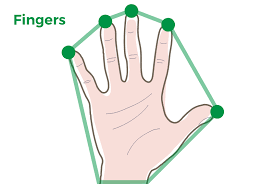
\includegraphics[width=0.5\textwidth]{IMG/HandSens.png}
\captionof{figure}{Visualization of hand recognition software}
\end{center}

\indent Microsoft released another interpretation of a motion sensing input design with the Xbox Kinect \cite{kinect}. The device includes an additional IR light source and an infrared camera for depth mapping and an RGB color VGA video camera for image recognition. The camera is capable of isolating the human from the background and with image recognition track individual limbs. The Microsoft SDK package for the system also includes access to the massive database for image recognition. This has been shown to work with small children using sign language learning software.

Plenty of other approaches also exist. One of the most popular is the usage of flex sensors. The concept is very simple, a change of resistance occurs with deflection, ie the flexing of a joint. The main disadvantage of such a solution is very low cost/efficiency ratio. However this method takes up very little space and low power consumption.

Another accurate positioning method is with the use of multiple MPUs placed in carefully selected positions. If connected via a I2C protocol we may connect many along a single bus. These sensors are quite inexpensive compared to the flex sensor and provide acceptable accuracy when paired with suitable filters such as a Kalman filter. If not taken into account, the position obtained drifts over time resulting in a high error. However this can easily be mitigated.

With a strategically placed camera and a line emitting IR blaster we may create a vision system that proves to be much more reliable than the previous concept. DIGITS \cite{Digits} is the realization of such a device. It is capable of emulating the human hand in a virtual environment with great success.

\begin{center}
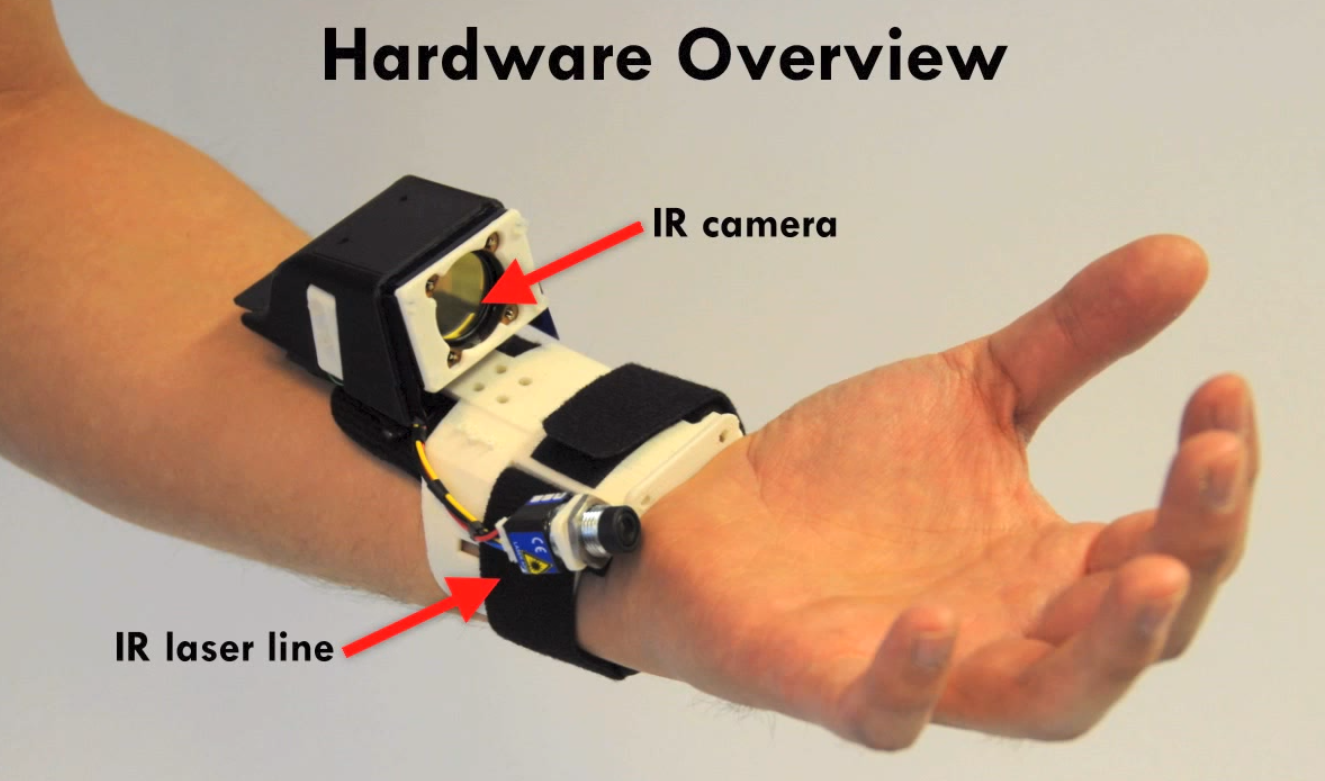
\includegraphics[width=0.5\textwidth]{IMG/HandSens02.png}
\captionof{figure}{A finger position method by Digits \cite{Digits}}
\end{center}

\indent The IR blaster greatly increases the image recognition performance by giving it obvious vision cues. The wrist mounted device may also benefit from an additional MPU sensor that will provide us with information on the placement of the arm. Such a system is not limited by the environment; lighting levels and surrounding colors wouldn't have a significant impact on the performance of the mechanism.

\subsection{Control}

For an electronic control system we may consider two distinct architectures that will be ideal for our device; an FPGA board or a microcomputer like the Raspberry Pi. Both devices are capable of image signal processing with the use of the OpenCV library, therefore all techniques discussed above are viable. In extension, OpenCL (an official and supported extension to OpenCV) can be used inplace of HDL in FPGA to improve design productivity. The main advantage of FPGA over a CPU is parallelism\cite{FPGA}. In a system where many sensors and actuators are present, and a quick response of a mechanical hand is essential this can become a major advantage over traditional microcomputers. However, this comes with a cost of complexity.

Both systems are also capable of signal filtering and noise reduction. This can reduce micro motions and sensor imperfections to create a much more fluid movement of the hand. Additionally, machine learning could incorporate a decision making process that could create precise maneuvers even if the operator isn't fully trained or capable of them.  Potentially becoming an enhanced extension of the human by providing stability and limiting the motion to avoid accidental jerks or unwanted reflexes.

\section{Concept}
\subsection{Mechanics}

The primary attributes of our mechanical hand will be its gripping capabilities and precision. To achieve this while keeping the entire project within acceptable dimensions we need to introduce dependent joints with certain flexion compliance.

Some of the dependent joints will have an additional mechanism extended from it. This mechanism will usually consist of a spring that is pushing on a lever. With no external forces, the lever will be sitting in a locked maximum position. The moment it comes into contact with something and depending on the amount of force applied, the lever hinges back. This gives the dependent joint a certain amount of restricted movement that mimics the joints of the hand in a similar fashion. This sort of compliance will greatly increase the hands holding capabilities by being able to mechanically adapt to the objects geometrical features.

A single hand will be comprised of three digits, each with two degrees of controlled motion. However, due to flexion compliance it will have many more degrees of freedom. The human hand has four bones for each finger and three for the thumb. The bones go as follows from the tip of the finger to the wrist; distal phalanges, medial phalanges, proximal phalanges and the metacarpals. With the thumb lacking the medial phalanges. Each finger has four degrees of freedom except for the thumb by only having three. Next we will explore all our joints and describe how we plan to resolve them. 

The first is the opposable thumb, which will have two joints and one degree of controlled motion. The distal phalanges will have flexion compliance, while the metacarpal will be driven by a larger motor to match the cumulative force of the other joints. The thumb needs to be as universal as its counterpart. Both grip strength and precision tasks paired with the other fingers are important. 

The index finger will have four joints and also two degrees of motion. The distal phalanges will have 90 degree flexion compliance and is dependent on the angle of the medial phalanges. The medial phalanges and proximal phalanges will be each driven by a motor, while the metacarpals will be attached by ball joint and given minimal flexion compliance.

The final three fingers will be combined into one larger finger. Since these fingers are usually used for gripping and handling of objects, they will be mounted with larger motors and the larger surface area will provide a better gripping surface. The joint mobility will be similar to the index finger.

The last area to cover is the palm. The metacarpals is responsibly for its shape. We have two metacarpals that have flexion compliance and one on the thumb that is driven. This means the palm has the capability of adjusting its shape to a gripped object.

\subsection{Control and Sensors}

With the mechanical end of the project providing advantages gripping mechanisms and variable grip strength, the control of the device may be much more forgiving and the use of haptic feedback isn't as necessary. With this in mind, we may create a completely non invasive human operated controller with the use of vision systems.

The system will be made up of two cameras that will provide stereo vision. With proper calibration, we may produce a depth map and isolate a human operator from the background. Once isolated, it is a matter of manipulating the image and developing algorithms that may track geometrical features. Libraries such as OpenCV already provide most of these features in languages such as Python and C++.

The readings from the camera may be further improved by adding a layer of machine decision making. Certain filters for noise reduction are certainly necessary, however we may also include pre-programmed operations that may assist the human and become an extension of him. For instance, we may limit the velocity of fingers to reduce abrupt movements in certain situations or remember the gripping position for a certain object. This way the operator carries out the general movement required of the robot and the robot decides on the precise movements that may be difficult for the user to control. 

\subsection{Electronics and Actuating}

Since the image signals from two cameras have to be processed in real-time it is important to consider a capable computer. We decided that the entire Vision System will be run on Raspberry Pi 3 Model B microcomputer. This device possesses a quad-core 64bit processor and 1GB RAM, hence is capable of performing desired operations. Further reassurance of its capabilities is the many camera modules and OpenCV projects already developed for the Raspberry.

The robotic fingers will be actuated by six servomotors controlled by an Arduino Uno R3 attached to the hand. The Arduino Uno R3 has 14 digital input/output pins (of which 6 can be used as PWM outputs). The wireless connection between the Raspberry Pi 3 B and the Arduino will be implemented with the use of a Bluetooth protocol. The Raspberry has a built-in Bluetooth module and Arduino can be easily extended with a HC-0x series Bluetooth module.

The Arduino controller and motors will be energized by an individual power supply with a voltage stabilizer. The Raspberry Pi will be energized by a set of 18650 cells through a voltage stabilizer.

\break
\section{Software}
\subsection{Requirements}
Requirements analysis is the first stage in the systems engineering process and software development process. The software requirements specification (SRS) lays out functional and non-functional requirements, and may include a set of use-cases that describe user interactions that the software must provide. We will carry out such an analysis on our system.

The purpose of this software is simple, to track the movements of a human hand. Specifically, we need to obtain certain points correlated to the human hand that satisfy our kinematic equations. The system will have to operate in real time with minimal delays. This system must also be non-invasive and work reliable in many different environments. Our solution implements a vision system. The general structure will look as such; capture footage, process the video feed, analyze the data and implement filters or statistical methods to improve the tracking. The product must work with minimum product knowledge, so called plug-and-play.

The user will interact with the system through both the vision system and voice controls. The camera system will be operating at a distance from the user, therefore to implement a user interface that is convenient to use and continues to be non-invasive and non-contact, as the hands are preoccupied, we will be relying on voice actuation. This will provide basic functionality on top of the core tracking service. 

We will also be communicating with another device, which in turn is responsible for controlling the mechanical hand. The information processed by our software will provide the secondary device with the information it needs to carry out the inverse kinematic calculations. This information will be in the form of coordinate points. This process must be robust with very fast response time. The quality of the point detection must be reliable and stable. It must also be tolerant to any user mistakes.

Additional limitations to our software will involve the hardware it will be run on. Our system will be limited to the capabilities of the Raspberry Pi, as well as the available libraries. Our vision system will be built on the OpenCv library, while our voice actuation on the Sphinx libraries. Both libraries support C++ and Java.\vspace{12pt}

The software aims to provide natural control for complex end-effectors. The human brain is very good at calculating inverse kinematics of its own body, to the point where it is completely natural to us without much thought. By taking advantage of this, we may quicken the learning process for controlling advanced machinery and allow for much more complex maneuverability. Controlling a mechanical hand is one possible use-case, however by selecting what points and how many points are to be tracked, this software may be used for many different types of control, not necessarily mechanical. The software may be just as easily used for gesture control or interpreting sign language. Extensibility needs to be considered during the design process. Additionally, we may provide options for several different supported cameras and tracking modules and expand these features over time with software updates.

\subsection{Implementation}
We may break our entire software apart into several subcategories; vision system, vision system calibration, audio system and audio system calibration. The calibration software will be used by the developers to prepare certain models to work with our software, this will be discussed in much more detail below. The user will be interacting exclusively with our vision and audio software.
\subsubsection{Vision System Calibration}
The calibration process is made up of several key steps depending on the technology used. First let us look at the calibration of a stereo camera setup for the creation of disparity maps. We begin by calculating the intrinsic parameters of each camera, this includes the focal length, principle points and consequently the distortion coefficients. We use this information to undistort each individual camera. Following this, we need to calculate the extrinsic parameters. During this process we acquire information of where one camera is with respect to the other, this includes the rotation and translation matrix. From this we additionally acquire the fundamental and essential matrix, which in turn gives us the rectification parameters. After rectifying the images, we will have matching epipolar lines in each camera and we may begin the disparity mapping process. The disparity map gives us clear information on the hands location and its shape. The actual tracking software will be discussed later.

\begin{figure}[!hb]
    \begin{minipage}[b]{0.49\textwidth}
    	   \centering
		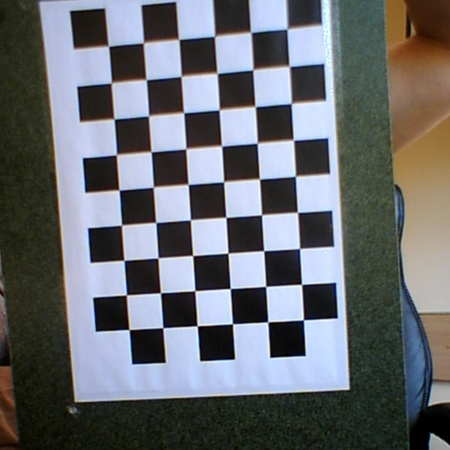
\includegraphics[width=\textwidth]{IMG/Cal_01.jpg}
		\captionof{figure}{Calibration Image}
	\end{minipage}
    \hfill
    \begin{minipage}[b]{0.49\textwidth}
	    \centering
		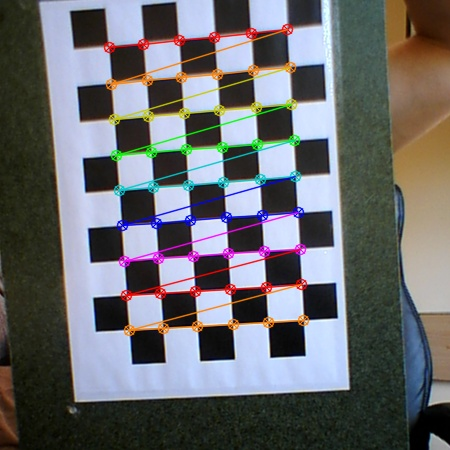
\includegraphics[width=\textwidth]{IMG/Cal_02.jpg}
		\captionof{figure}{Calibration Image With Overlay}    	
	\end{minipage}
\end{figure}

In the case of an IR blaster setup, the calibration will look slightly different. Since we will only be using one camera to create a disparity map, the calibration will be much simpler. After calculating the intrinsic parameters, the camera should be ready.
\subsubsection{Vision System}
The vision system will be comprised of several steps. The first being to discern the hand from other objects and background noise. This will be done with the use of disparity maps and thresholds. After obtaining a clearly defined silhouette of the object to be tracked, we focus on the original video feed again and pattern the singled out area with a grid of points. These points will be used in our Lucas-Kanade tracking algorithm that will create optical flow vectors for each of the given points. This will provide us with displacement and velocity information. The next step requires another set of algorithms that first filter any errors in the optical flow map and then using statistical methods returns a few individual points that correspond to the hands position in 3D space.


\begin{center}
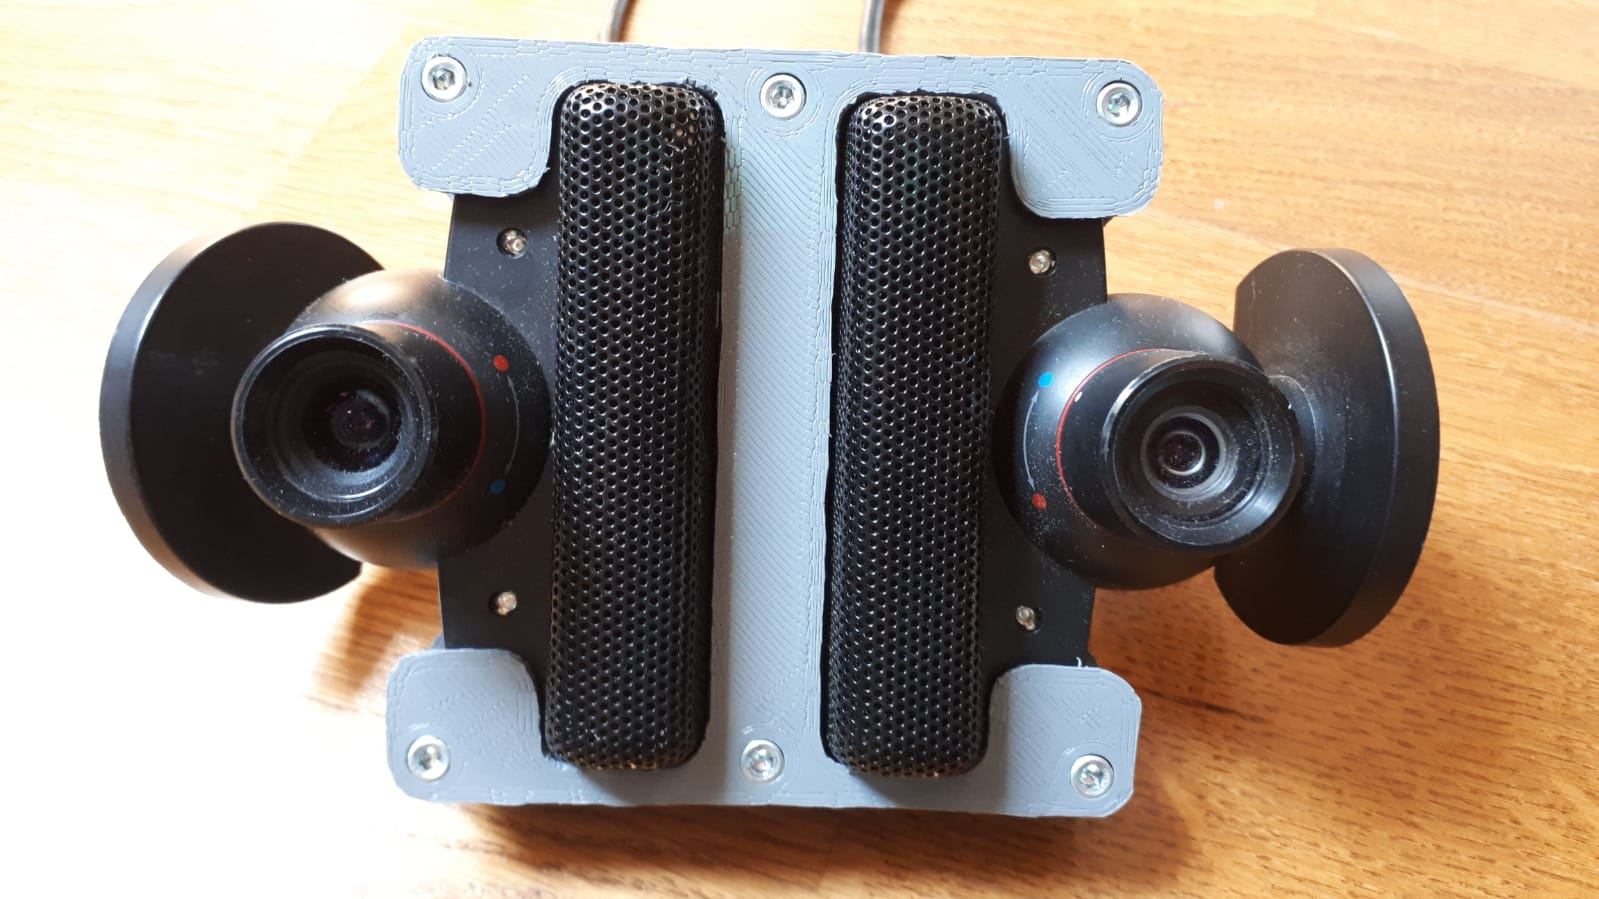
\includegraphics[width=0.5\textwidth]{IMG/DualCam.jpeg}
\captionof{figure}{Dual Camera Setup}	

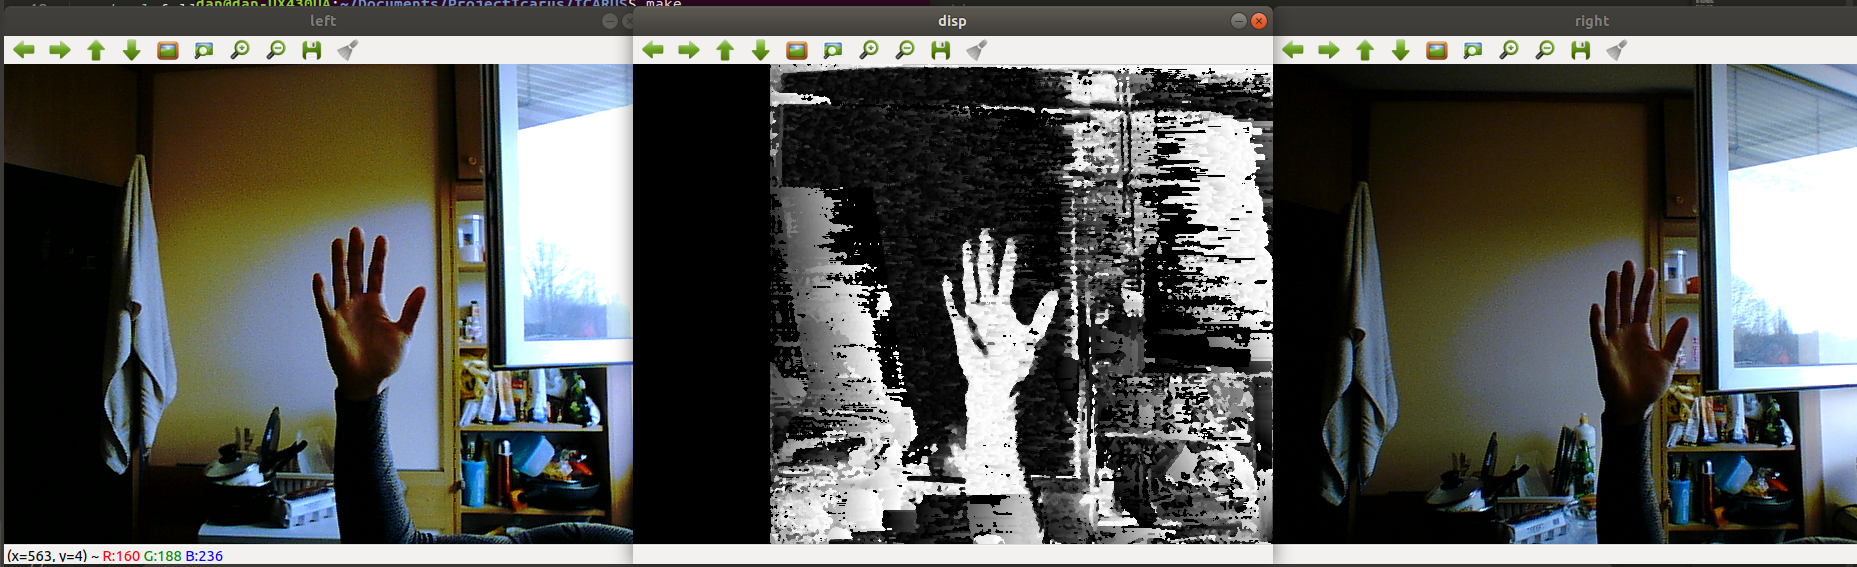
\includegraphics[width=\textwidth]{IMG/DualCam_Disp.PNG}
\captionof{figure}{Disparity Map}   	
\end{center}

\subsubsection{Audio System}
The general process of the application consists of several key steps. We begin with interval audio recordings. After each interval recording, it decodes the .raw file and searches for a keyword. If the keyword was spoken, the recording re-initiates. The second .raw file is decoded to receive a string. This string needs to be compared to the applications look up table. The final part is the calling of the function which is most appropriate based on the returned string. 
Many other classes make up the individual actions of the application. These “action” classes are very easy to add and are what makes the program modular. 
To accomplish all of this we needed to take advantage of language and audio processing API’s. These are briefly introduced and summarized below:

\paragraph{PocketSphinx}
Pocket-Sphinx is a lightweight speech recognition engine, specifically tuned for handheld and mobile devices. The libraries are written in C and are dependent on the Sphinx-Base library. \vspace{12pt}

\noindent For the library to function properly, we need to provide additional models and dictionaries:
\begin{itemize}
	\item Acoustic model: The acoustic model models the sound of a phone, it translates recorded sounds into labeled phones. Usually a hmm is used. Each phone has a hmm. 
	\item Phonetic dictionary: Maps phones to words.
	\item Language model: Used to determine sequences of words that are allowed. 
\end{itemize}
	

\noindent Most models require training to be more accurate:
\begin{enumerate}
	\item Acoustic models require lots of recordings of people saying words and sentences (not that difficult to do) and accurate transcription of the recordings (time consuming). It is possible to take an existing model and quickly adapt it to a particular speaker.
	\item Language models require for different systems different language models. Different applications need to recognize different sets of words.
	\item The performance of the recognizer is significantly improved if your language model only considers relevant words to your application.
	\item You can take an existing language model and trim it to what you need, or make on from scratch using the JSGF format.
\end{enumerate}
	


Words are a sequences of sounds, where each sound is a phone. However, the exact pronunciation of a phone depends on the phones before and after.
Diphones are two phones. Diphones are less impacted by the phones that come before or after. 
Senones are triphones and quinphones.
While there are many phones, not all combinations of a phone is a word. Thus, we should not simply recognize phones, but we need to recognize words which are sequences of phones.
Besides phones are fillers (ex., breath, “um”). An utterance is a sequence of words and fillers. Utterances are separated by a pause.



\paragraph{ALSA(Advanced Linux Sound Architecture)}
Sound is converted to its electrical form by a transducer, such as a microphone. An analog-to-digital converter (ADC) converts the analog voltages into discrete values, called samples, at regular intervals in time, known as the sampling rate. By sending the samples to a digital-to-analog converter and an output transducer, such as a loudspeaker, the original sound can be reproduced.

The size of the samples, expressed in bits, is one factor that determines how accurately the sound is represented in digital form. The other major factor affecting sound quality is the sampling rate. The Nyquist Theorem states that the highest frequency that can be represented accurately is at most one-half the sampling rate. 

We will mostly be interested in the PCM interface: the interface for managing digital audio capture and playback. 

 A sound card has a hardware buffer that stores recorded samples. When the buffer is sufficiently full, it generates an interrupt. The kernel sound driver then uses direct memory access (DMA) to transfer samples to an application buffer in memory. Similarly, for playback, another application buffer is transferred from memory to the sound card's hardware buffer using DMA.
 
These hardware buffers are ring buffers, meaning the data wraps back to the start when the end of the buffer is reached. A pointer is maintained to keep track of the current positions in both the hardware buffer and the application buffer. Outside of the kernel, only the application buffer is of interest, so from here on we discuss only the application buffer.
The size of the buffer can be programmed by ALSA library calls. The buffer can be quite large, and transferring it in one operation could result in unacceptable delays, called latency. To solve this, ALSA splits the buffer up into a series of periods and transfers the data in units of a period.
A period stores frames, each of which contains the samples captured at one point in time. For a stereo device, the frame would contain samples for two channels.

\begin{figure}[!hb]
    \begin{minipage}[b]{0.49\textwidth}
    	\centering
		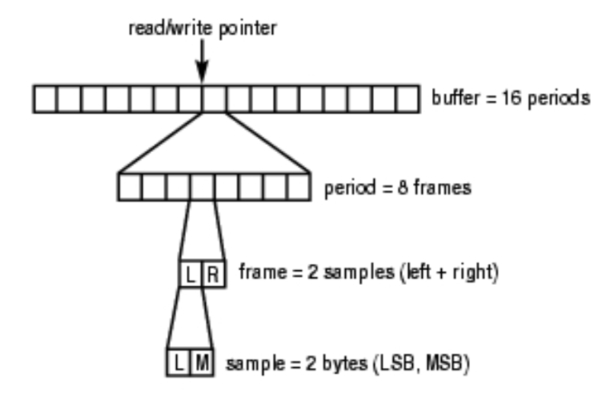
\includegraphics[width=0.8\textwidth]{IMG/ALSA.PNG}   	
	\end{minipage}
    \hfill
    \begin{minipage}[b]{0.49\textwidth}
		The Application Buffer (Over and Under Run), illustrates the breakdown of a buffer into periods, frames and samples with some hypothetical values. Here, left and right channel information is stored alternately within a frame; this is called interleaved mode. A non-interleaved mode, where all the sample data for one channel is stored followed by the data for the next channel, also is supported. 	
		\captionof{figure}{}   	
	\end{minipage}
\end{figure}





When a sound device is active, data is transferred continuously between the hardware and application buffers. In the case of data capture (recording), if the application does not read the data in the buffer rapidly enough, the circular buffer is overwritten with new data. The resulting data loss is known as overrun. During playback, if the application does not pass data into the buffer quickly enough, it becomes starved for data, resulting in an error called underrun. The ALSA documentation sometimes refers to both of these conditions using the term XRUN. Properly designed applications can minimize XRUN and recover if it occurs.

\noindent Programs that use the PCM interface generally follow this pseudo-code:
\begin{itemize}
	\item open interface for capture or playback
	\item set hardware parameters (access mode, data format, channels, rate, etc.)
	\item while there is data to be processed:
	\begin{itemize}
		\item read PCM data (capture)
		\item write PCM data (playback)
	\end{itemize}
	\item close interface
\end{itemize}
	
When we open the PCM stream, we specify the mode as SND\textunderscore PC\textunderscore STREAM\textunderscore CAPTURE. In the main processing loop, we read the samples from the sound hardware using snd\textunderscore pcm\textunderscore readi and write it to standard output using write. 

In order to set the hardware parameters for the stream, we need to allocate a variable of type snd\textunderscore pcm\textunderscore hw\textunderscore params\textunderscore t. We do this with the macro snd\textunderscore pcm\textunderscore hw\textunderscore params\textunderscore alloca. Next, we initialize the variable using the function snd\textunderscore pcm\textunderscore hw\textunderscore params\textunderscore any, passing the previously opened PCM stream. 

We now set the desired hardware parameters using API calls that take the PCM stream handle, the hardware parameters structure and the parameter value. We set the stream to interleaved mode, 16-bit sample size, 1 channel and a 44,100 bps sampling rate. In the case of the sampling rate, sound hardware is not always able to support every sampling rate exactly. We use the function snd\textunderscore pcm\textunderscore hw\textunderscore params\textunderscore set\textunderscore rate\textunderscore near to request the nearest supported sampling rate to the requested value. The hardware parameters are not actually made active until we call the function snd\textunderscore pcm\textunderscore hw\textunderscore params.

\section{Kinematics}
\subsection{Index Finger}
We will begin the analysis with the index finger. The mechanical finger may be represented by a simplified kinematic model presented below. Our system has two degrees of freedom, however the structure is much more complicated due to various lever systems and dependent angles. To simplify our mechanism, we may divide the system into four subsystems. Each system will have its own set of equations that will eventually be put together in a programming environment to define the movement of the finger.

\begin{center}
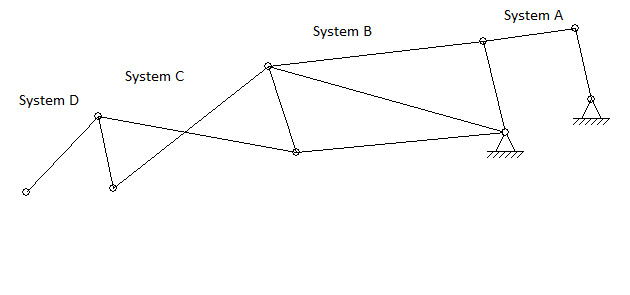
\includegraphics[width=0.7\textwidth]{IMG/IK_01.jpeg}
\captionof{figure}{Kinematic Model}	   	
\end{center}

Inverse kinematics for system A. This system is a simple 4 bar linkage mechanism that consists of a crank, coupler, rocker and frame. The motor attaches to the crank and drives the proximal phalange. The motor angle $\varphi$ drives $\alpha$, therefore the inverse kinematic formula has only one unknown variable $\alpha$ that is provided by system B. The rest of the formula consists of constants that are properties of the system. \textbf{\textit{All calculations are provided in the appendix.}}

\begin{center}
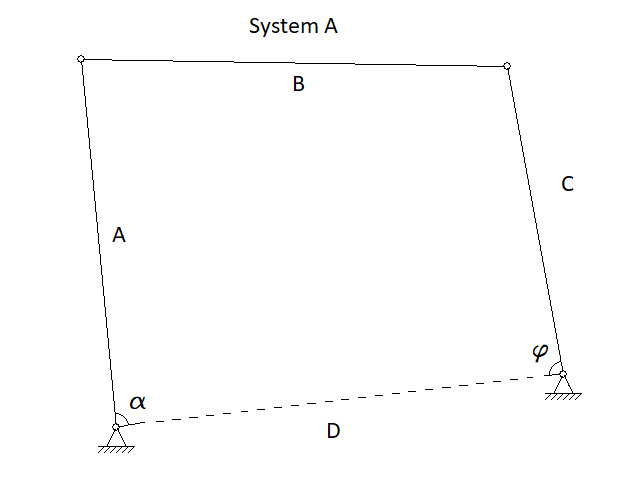
\includegraphics[width=0.45\textwidth]{IMG/IK_02.jpeg}
\captionof{figure}{4 bar linkage mechanism}	   	
\end{center}

\[ \varphi = sin^{-1} \bigg(\frac{Asin\alpha}{\sqrt{A^2+D^2-2ADcos\alpha}}\bigg) + cos^{-1} \bigg(\frac{A^2+D^2-2ADcos\alpha-B^2+C^2}{2C\sqrt{A^2+D^2-2ADcos\alpha}}\bigg)\]

Inverse kinematics for system B. This is the simplest possible system being a simple lever. However due to the software constraints, we have to additionally consider the orientation of the base coordinate system (the palm) and the offset from the motors 0 degree position. The formula is provided with the X coordinate from the camera system and based on this information figures out the angle on the four bar linkage mechanism.

\begin{center}
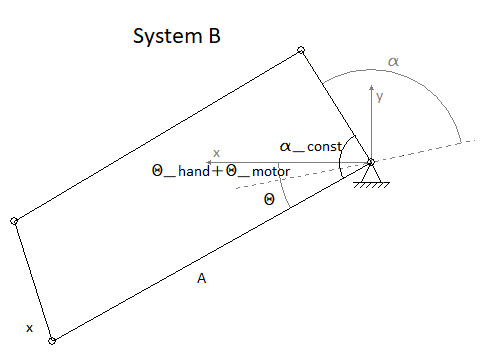
\includegraphics[width=0.5\textwidth]{IMG/IK_03.jpeg}
\captionof{figure}{Proximal Phalange}	   	
\end{center}

\[ \alpha = cos^{-1}\bigg(\frac{X}{A}\bigg) - (\theta_{hand} + \theta_{motor}) + (\pi - \alpha_{const}) \]

Provided the two equation above, we have everything we need to control the proximal phalange with the first servo motor. The servo motor is controlled entirely by one X axis coordinate provided by the software. The equations take into account various offsets, such as the orientation of the palm, as well as properties of the system such as orientation of the motor. To optimize the geometry, we may use the first equation to equate a certain rotation of the motor to the angular displacement of the finger.\vspace{12pt}

The second part of the finger is much more complicated. The mechanism is a crossed four bar linkage, which significantly complicates the equations. First we will provide several formulas that create dependencies between various angles of the mechanism.

\begin{center}
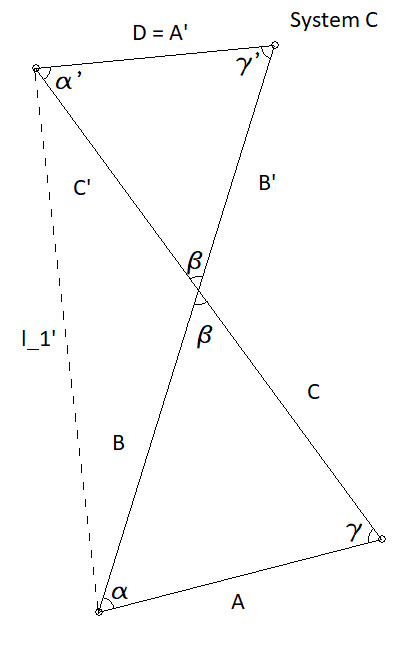
\includegraphics[width=0.28\textwidth]{IMG/IK_04.jpeg}
\captionof{figure}{Crossed 4 bar linkage mechanism}	   	
\end{center}


This formula provides us with the length the driving string needs to shorten. The only unknown is $\gamma$.
\[ l_1' = \sqrt{A^2+C^2-2ACcos\gamma}\]

This formula is taken as a proportion of the two triangles formed by the crossed mechanism. It helps us relate opposite angles.
\[ C' = \frac{CA'}{A} \frac{sin\gamma'}{sin\gamma} \]

Based on the equations above and a few more tricks, we are able to relate both angles from one side of the crossed four bar linkage mechanism. At this point we have all the information required to continue our calculations.
\[ \gamma' = cos^{-1}\bigg( \frac{-A^2+B^2-C^2+D^2+2ACcos\gamma}{-2CD} \bigg)\]

\[ \alpha = sin^{-1} \bigg( \sqrt{\frac{Bsin\gamma-(C-C')sin\gamma'}{C'}} \bigg) \]

The formula above may be used for an inverse kinematic system for the medial phalange, which is what is included in the Arduino. The last formula is much too complicated to derive for an inverse kinematic system, therefore a numeric solution is necessary. With the forward kinematic equation below, we may create a look up table and relate both $\gamma'$ and $\alpha$ to $\gamma$ which in turn provides us with the necessary information to calculate the shortening of the string and movement of the motor.

\begin{center}
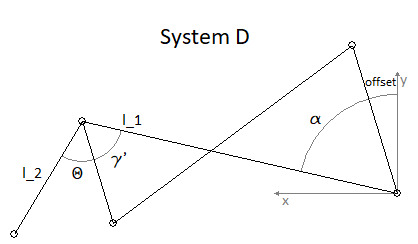
\includegraphics[width=0.5\textwidth]{IMG/IK_05.jpeg}
\captionof{figure}{Distal Phalange}	   	
\end{center}


\[ X = l_1 cos(\alpha+offsets) - l_2 cos(\gamma') \]


\subsection{Thumb}

\subsection{Arduino}
The formulas derived earlier are for the purpose of controlling the hand, therefore they need a controller. The Arduino Nano is the board of choice being that it is very similar to the Arduino UNO (where all the testing was done) and is very compact. The Atmega328's 8-bit CPU running at 16MHz is more than sufficient for calculating our equations in real time. The Nano has only 6 PWM pins, however the provided servo libraries support many more. A servo only requires a pulse 1ms long, so a driving frequency of 1kHz. Such a frequency is easily accomplished by the integrated CPU and we may actually use any of the outputs on the device. The 14 digital pins and 8 analog summed up for a total of 22 pins is more than sufficient for wiring up our device. The servo motors are powered by an external power supply, therefore the Arduino Nano has the sole task of controlling the motors.

\begin{center}
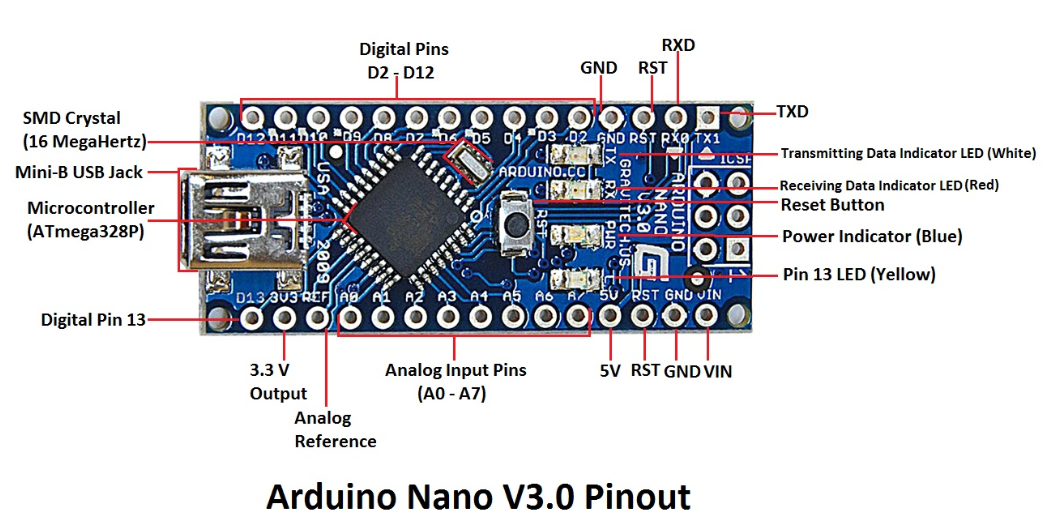
\includegraphics[width=\textwidth]{IMG/Nano.png}
\end{center}

An external device will provide the parameters necessary for our equations. We will  now review the code structure. For each motor, there exists a separate INO file that contains all the necessary equations and conversions in reusable methods. This allows us to reuse many of the formulas. Additionally, there exist parameter files that carry the mechanisms properties. 


\break
\begin{thebibliography}{1}
	\bibitem{bebionic} BeBionic. Retrieved from {\url{http://bebionic.com/the_hand/technical_information/}} 
	\bibitem{vincent} VincentSystems. Retrieved from {\url{  https://vincentsystems.de/en/}} 
	\bibitem{JRRD} U.S. Department of Veterans Affairs, {\em Journal of Rehabilitation Research And Development}. Volume 50 Number 5, 2013
   Pages 599-618 Retrieved form {\url{https://www.rehab.research.va.gov/jour/2013/505/page599.html}}
	\bibitem{stringHand} SOLIDWORKS. Retrieved from {\url{ http://blogs.solidworks.com/tech/2016/08/solidworks-time-lapse-tutorial-mechanical-hand.html}}
	\bibitem{airMuscle} Peter Scarfe, Euan Lindsay {\em Air Muscle Actuated Low Cost Humanoid Hand}. Retrieved from {\url{ http://cdn.intechopen.com/pdfs/4176/InTech-Air_muscle_actuated_low_cost_humanoid_hand.pdf
}} 
	\bibitem{kinect} Kinect. Retrieved from {\url{https://www.jameco.com/jameco/workshop/howitworks/xboxkinect.html}}
	\bibitem{Digits} DIGITS. Retrieved from {\url{https://spectrum.ieee.org/video/consumer-electronics/audiovideo/digits-hands-free-3d}}	
	\bibitem{ALTERA} Altera, Video and Image Processing Design Using FPGAs. Retrieved from {\url{https://www.altera.com/en_US/pdfs/literature/wp/wp-video0306.pdf}}
	\bibitem{CpuFpga} Brandon Treece ,VisionSystems Design. Retrieved from {\url{https://www.vision-systems.com/articles/print/volume-22/issue-8/features/cpu-or-fpga-for-image-processing-which-is-best.html	}}
	\bibitem{FPGA} FPGA in Robotics. Retrieved from {\url{https://robotics.stackexchange.com/questions/1153/when-should-fpgas-be-used-in-robotics}}
	\bibitem{CpuFpga02} APUs vs FPGAs. Retrieved from {\url{http://www.electronicdesign.com/microprocessors/apus-vs-fpgas-battle-smart-camera-processing-supremacy}}
	\bibitem{Intel} Intel FPGA SDK for OpenCL. Retrieved from {\url{https://www.altera.com/en_US/pdfs/literature/hb/opencl-sdk/aocl_programming_guide.pdf}}
	\bibitem{OpenCL} OpenCL. Retrieved from {\url{https://opencv.org/platforms/opencl.html}}
	\bibitem{VisionProcessing} Video and Image Processing Suite Intel FPGA IP. Retrieved from {\url{https://www.altera.com/products/intellectual-property/ip/dsp/m-alt-vipsuite.html}}
	\bibitem{Grip} A comparison of the grip force distribution in natural hands and in prosthetic hands. Retrieved from {\url{https://pdfs.semanticscholar.org/f600/c0ad7d6ecb7510b1b8e8f1318ffa03bb48cd.pdf}}
	\bibitem{LK01} Lucas-Kanade Tutorial Example 1 Retrieved from {\url{https://www.mathworks.com/matlabcentral/fileexchange/48744-lucas-kanade-tutorial-example-1?focused=3854179&tab=example}}, version 1.0 by Zhiyuan



\end{thebibliography}
  
\end{document}